\section{Analysis}
\label{sec:Analysis}

The absolute uncertainty of the counting rates, that were measured in this experiment are calculated with the formula 
\begin{align}
    \Delta N = \sqrt{N} \implies \Delta A = \sqrt{\frac{A}{\Delta t}} \, ,
\end{align}
because $N$ is poisson-distributed.
% End of Error Calculation

\subsection{Signal Shape}

The shape of the signal after the amplifier is shown in \autoref{fig:shapeofyou}. 
The comparison with the signal before the amplifier and after the pre-amplifier is not possible, because of noise, no common shape was recognizable.

\begin{figure}[htbp]
    \centering
    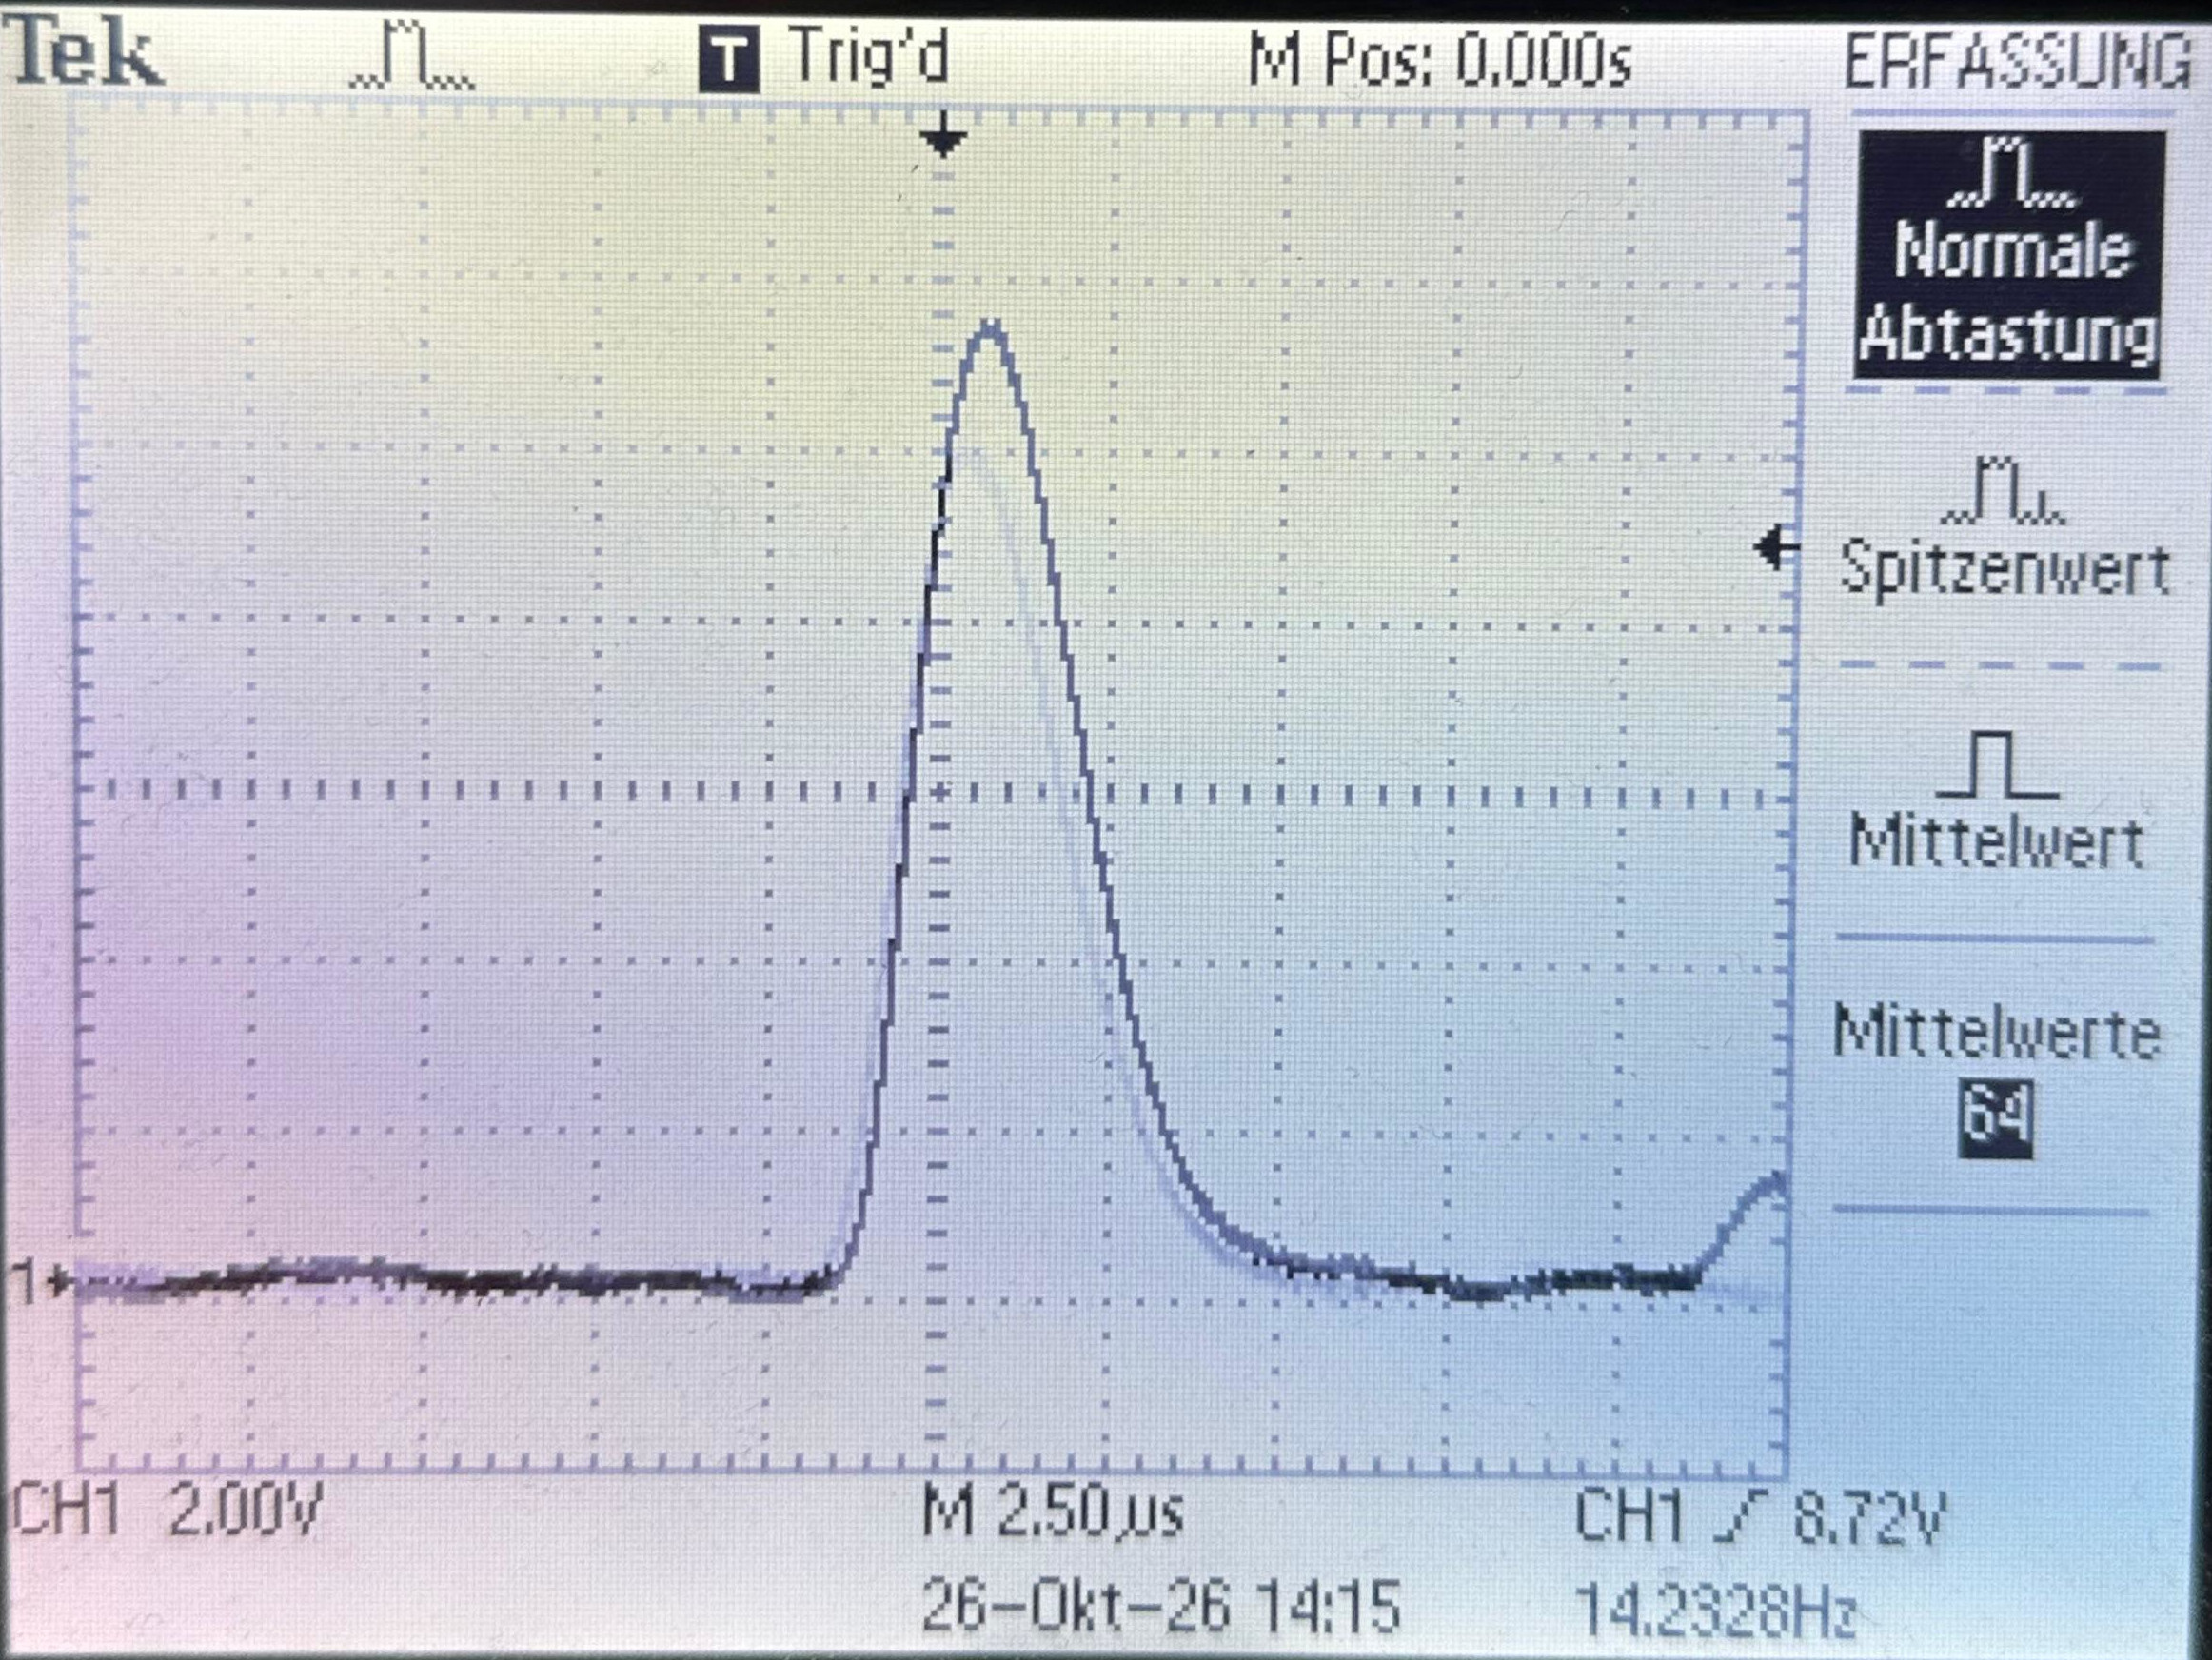
\includegraphics[width=0.8\textwidth]{content/pics/oszi.jpeg}
    \caption{Shape of the signal after the amplifier.}
    \label{fig:shapeofyou}
\end{figure}

\subsection{Callibration of the Solid-Angle Measurement}

To callibrate the zero point in the solid angle measuring apparatus, the measured counting rates from~\autoref{tab:small_angles} are being shown in~\autoref{fig:small_angles}. \\
The zero point $\Theta_0 = 0.5^{\circ}$ was selected, based on it being the highest measured count rate. 
Using \textit{curve\_fit} from \textit{Scipy}~\cite{scipy} a gaussian fit was implemented and it shows that actually the most optimal Zero-Point would have been $\Theta_0^{\text{opt}} = 1.45^{\circ}$.

\begin{figure}[htbp]
    \centering
    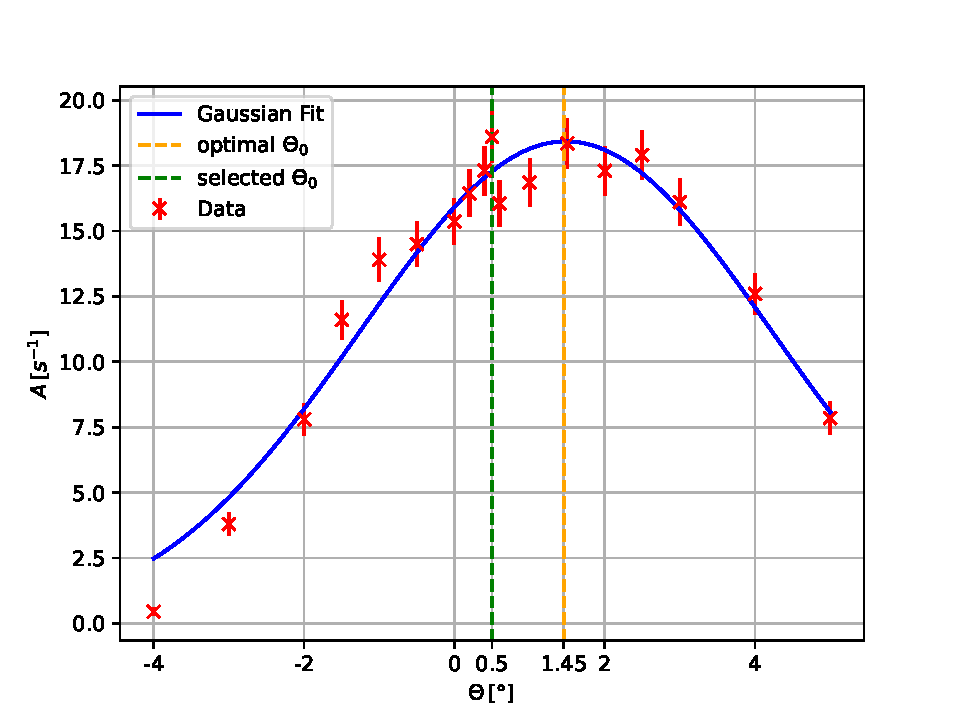
\includegraphics[width=0.75\textwidth]{content/plots/small_angles.pdf}
    \caption{Measured count rates $A$ plotted against the solid angle $\Theta$. The selected Zero-Point $\Theta_0$, as well as the optimal $\Theta_0$ - based on a gaussian Fit - have been plotted as well.}
    \label{fig:small_angles}
\end{figure}

% \clearpage
% \hspace{1cm}
\subsection{Examination of the Rutherford Scattering}

With the Zero-point being selected as $\Theta_0 = 0.5^{\circ}$ with $\Theta$ from \autoref{tab:small_angles}, the counting rates $A$ for bigger angles were measured and are being shown in \autoref{tab:big_angles}. 
In order to compare with the theoretical Rutherford Cross-Section~\eqref{eqn:rut} a fit of the form 
\begin{equation}
    A(\Theta) = \frac{\alpha}{\sin(\frac{\Theta}{2})^4} + \beta 
    \label{eq:fit_ruth}
\end{equation}
with $\alpha, \beta \in \mathcal{R}$ was being done using \textit{curve\_fit}~\cite{scipy}. \\

The fit yields the fitparameters 
\begin{align*}
    \alpha &= \qty{1.9(0.2)e-5}{s^{-1}}, & \beta &= \qty{0.79(0.23)}{s^{-1}} \, .
\end{align*}
In \autoref{fig:big_angles} a plot of the experimental data and the fit is to be seen. 
The observed fit curve seems a bit off, as the curvature sets in earlier than the experimental data suggests.

\begin{figure}[htbp]
    \centering
    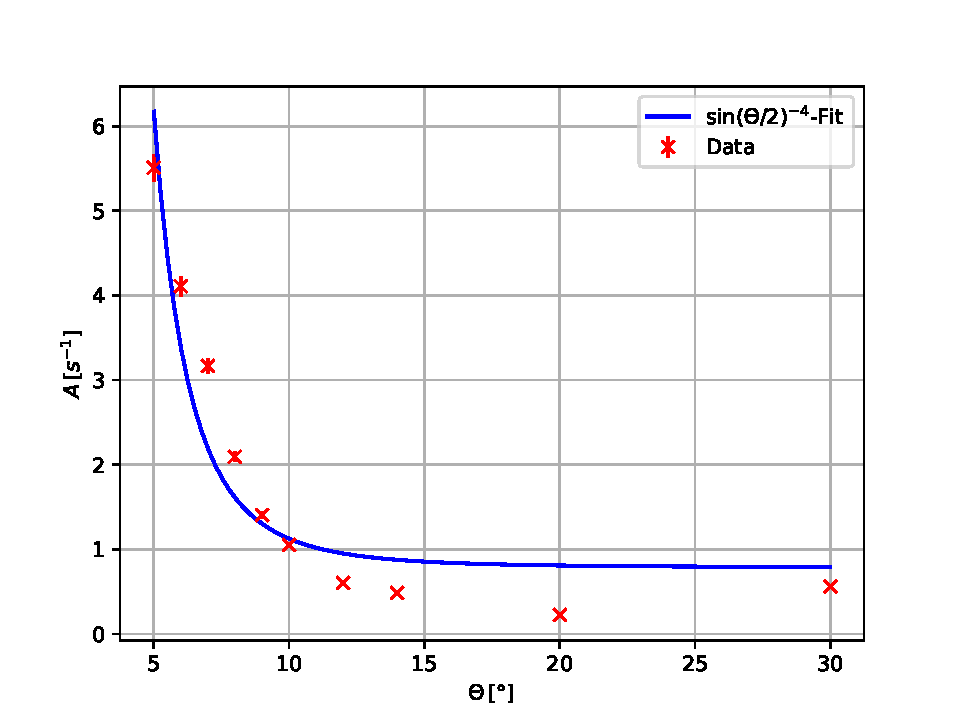
\includegraphics[width=0.75\textwidth]{content/plots/big_angles.pdf}
    \caption{Measured count rates $A$ plotted against the solid angle $\Theta$ and the fit function~\eqref{eq:fit_ruth}.}
    \label{fig:big_angles}
\end{figure}

This can however be treated by introducing the possibility of the Zero-Point of $\Theta$ not being aligned perfectly in the fit. 
The resulting fit of the modified fit function 
\begin{equation}
    A_\T{mod}(\Theta) = \frac{\alpha}{\sin(\frac{\Theta - \Theta_0}{2})^4} + \beta~\label{eq:mod_fit_ruth} \, ,
\end{equation}
is being shown in \autoref{fig:big_angles_mod}.
The fitparameters of the modified fit function are
\begin{align}
    \alpha &= \qty{3.2(1.6)e-5}{s^{-1}}, & \beta &= \qty{0.14(0.17)}{s^{-1}}, & \Theta_0 &= \qty{-5(1.2)}{^{\circ}} \, .
\end{align}

\begin{figure}[htbp]
    \centering
    \includegraphics[width=0.8\textwidth]{content/plots/big_angles_mod.pdf}
    \caption{Measured count rates $A$ plotted against the solid angle $\Theta$ and the modified fit~\eqref{eq:mod_fit_ruth}.}
    \label{fig:big_angles_mod}
\end{figure}

\subsection{Determining the foil thickness}

In order to determine the thickness of the foil, the dependence on the air pressure of the pulse height (which is proportional to the deposited energy) at the oscilloscope was measured. 
This was done in two measuring series, one with and one without the foil.
The data for that is found in~\autoref{tab:stopping_wof} and~\autoref{tab:stopping_wf} and visualized in~\autoref{fig:stopping_general}.

\begin{figure}[htbp]
    \centering
    \begin{subfigure}{0.49\textwidth}
        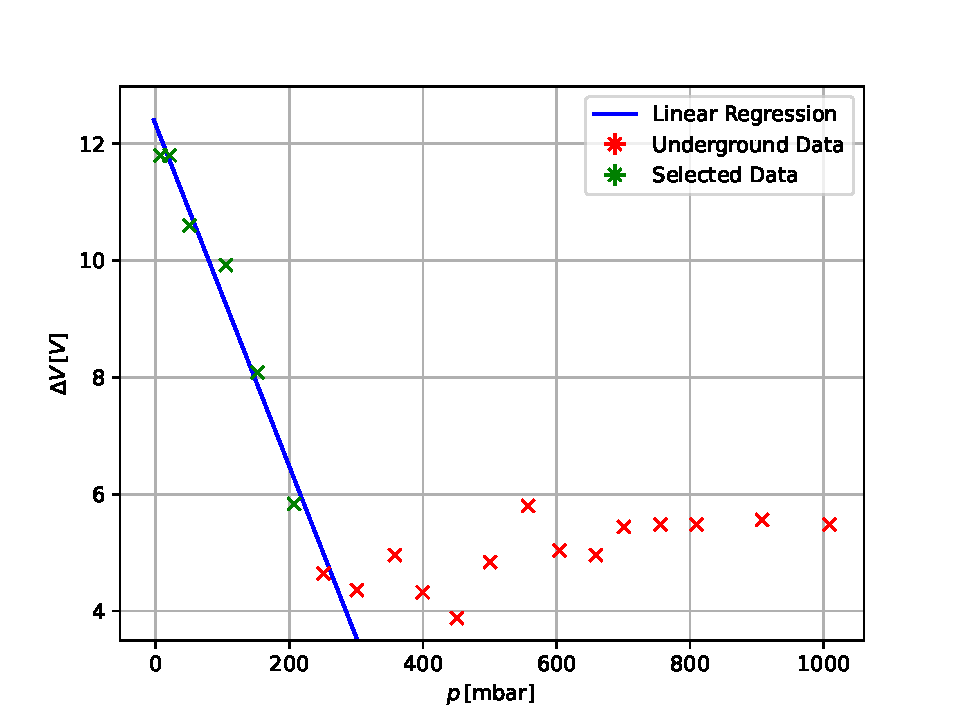
\includegraphics[width=\textwidth]{content/plots/stopping_air.pdf}
        \caption{Without gold foil.}
    \end{subfigure}
    \hfill
    \begin{subfigure}{0.49\textwidth}
        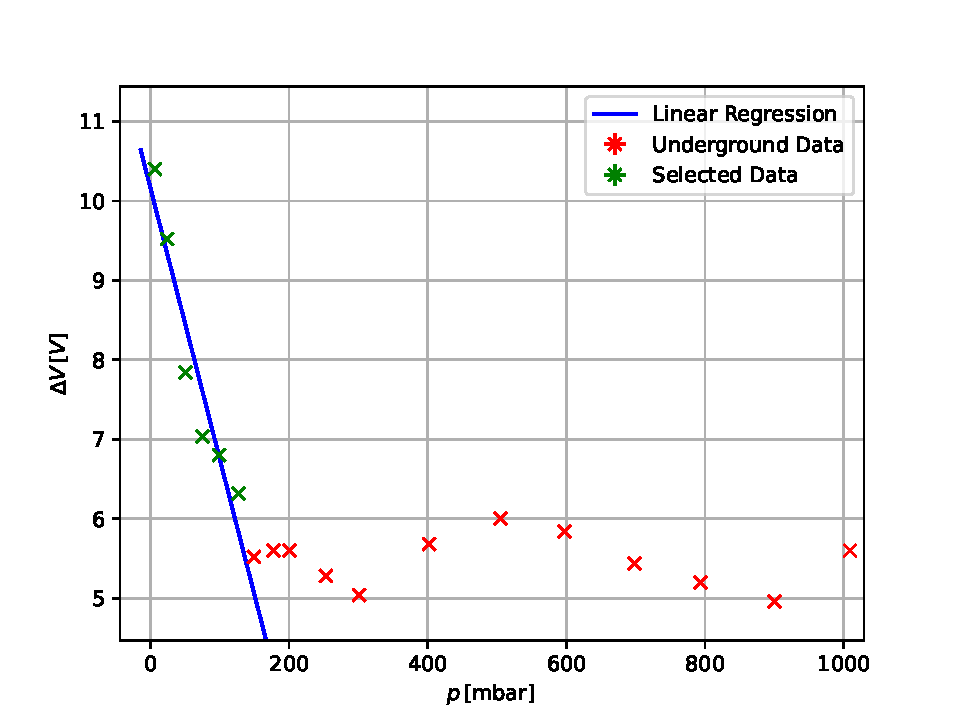
\includegraphics[width=\textwidth]{content/plots/stopping_gold.pdf}
        \caption{With gold foil.}
    \end{subfigure}
    \caption{Pulse height $\Delta V$ in dependence of pressure $p$ without foil (a) and with foil (b). Also a linear regression is performed.}
    \label{fig:stopping_general}
\end{figure}

For the lower pressures a linear regression using \textit{NumPy}~\cite{numpy} was performed. 
In order to understand why that was done, one has to look at the pressure dependence of the Bethe-Bloch-Formula~\eqref{eq:bethe}.
Using the ideal gas law, the density of target atoms $N$ can be written as 
\begin{align}
    N = \frac{pV}{k_B T}
\end{align} 
and hence
\begin{align}
    -\dif{E}{x} &= \frac{4\pi}{m_0 c^2} \frac{z^2}{\beta^2}\left(\frac{e^2}{4\pi\epsilon_0}\right)^2 \frac{p Z}{k_B T} \cdot \left[\ln\left(\frac{2 m_0 c^2 \beta^2}{I(1-\beta^2)}\right) - \beta^2\right] &\implies \dif{E}{x} &\propto -p \,.
\end{align}

For lower pressures the energy loss is therefore rather small and therefore the deposited energy can be approximated as 
\begin{align}
    \Delta E &\approx \dif{E}{x} \Delta x \propto -p \, ,
\end{align}
because the stopping power is rather constant over the length of energy deposition.
The measured pulse height therefore decreases in a linear fashion, until the range $R_\text{air}$ of the $\alpha$-particles in air decreases below the source-detector distance $L$, which means only some $\alpha$-particles hit the detector. \\
The reason why the measured curve does not decrease until zero will be discussed later, and for this analysis the plateau will be treated as an underground level on the oscilloscope.

The linear regression yields the following fitparameters, using the abbrevations (wf) $=$ ``with foil'' and (wof) $=$ ``without foil'':
\begin{align}
    m^{\mathrm{(wf)}} &= \qty{-34(5)e-2}{\volt\per\milli\bar}, & b^{\mathrm{(wf)}} &= \qty{10.2(0.4)}{\milli bar}, \\
    m^{\mathrm{(wof)}} &= \qty{-29(3)e-2}{\volt\per\milli\bar}, & b^{\mathrm{(wof)}} &= \qty{12.3(0.3)}{\milli bar} \, ,
\end{align}
with $m$ being the slope and $b$ being the $y$-axis intersection. 
Also the underground level is being evaluated at $V_0^{\mathrm{(wof)}} = \qty{5(0.5)}{\volt}$. \\

With that, the foil thickness can be calculated, by looking at the pulse height difference at $p = 0$. 
At that point, no $\alpha$-particle energy is being lost through interaction with the air molecules.
Hence, the difference in pulse height between the two curves with and without the foil is only explainable through the energy loss in the gold foil $\Delta E_\T{au}$. 
In other words the relation 
\begin{align}
    \Delta E_\T{au} = c \cdot \left(\Delta {V}^{\mathrm{(wof)}}(p=0) - \Delta V^{\mathrm{(wf)}}(p=0)\right) = c \Delta V(p=0)
\end{align}
with the conversion factor $c$ (between voltage measured from the Surface Barrier Detector and the deposited energy) must hold. 
For a sufficiently thin foil, the approximation $\Delta E_\T{au} \approx \dif{E}{x}|_\T{au} d_\T{au}$ is sufficable.
Using this and the linear regression, the foil thickness is determined through
\begin{align}
    d_\T{au} &= c \cdot \frac{b^{\mathrm{(wof)}} - b^{\mathrm{(wf)}}}{\dif{E}{x}|_\T{au}}~\label{eq:delta_x} \, .
\end{align}

As $\dif{E}{x}|_\T{foil}$ can be calculated using the Bethe-Bloch-Formula, the only missing factor is $c$. 
In order to obtain $c$, the slope of the linear regression without the foil can be examined:
\begin{align}
    \dif{E}{p} = c \cdot \dif{\Delta V}{p} = c \cdot m \implies \dif{}{p} \left(\dif{E}{x}|_\T{air} L \right) = mc~\label{eq:conversion} \, ,
\end{align}
in which $m = m^{\mathrm{(wof)}}$ and $L$ being the length between the detector and source.
$L$ can be extrapolated by looking at the pressure $p_\T{stop}$, where the slope in~\autoref{fig:stopping_general} intersects with the underground level. 
At that point, the range of the $\alpha$-particles should be exactly $L$ and since $R_\T{air} \propto (\dif{E}{x})^{-1} \propto p^{-1}$ the length $L$ can be calculated using
\begin{align}
    L = R_\T{air}(E_0, p_\T{stop}) = \frac{p_0}{p_\T{stop}} R_\T{air}(E_0, p_0) \, .
\end{align}

With 
\begin{align}
    p_0 &= \qty{1}{atm}, & p_\T{stop} = \frac{V_0^{\mathrm{(wof)}} - b^{\mathrm{(wof)}}}{m^{\mathrm{(wof)}}} &= \qty{250(30)}{\milli bar}, \\
    E_0 &= \qty{5.638}{MeV}\text{\cite{AtomkaerirekrCgibinNuclidenucAm241}}, & R_\T{air}(E_0, p_0) &= \qty{4.35}{\centi\meter}\text{\cite{astar}} \, ,
\end{align}
we get $L = \qty{17(2)}{\centi\meter}$. \\

Plugging $L$ and the values
\begin{align}
    z &= 2, & Z_\T{air} &= 14.46, & I &= \qty{16}{eV} \cdot Z^{0.9}\text{\cite{Povh1995}}, \\
    T &= 20^{\circ} C, & Z_\T{au} &= 79, & N_\T{au} = \frac{\rho_\T{au}}{m_\T{au}} &= \qty{5.9069e28}{m^{-3}}\text{\cite{CompositionGOLD}} \, ,
\end{align}
into the formula for $c$~\eqref{eq:conversion}, we get $c = \qty{0.45(0.04)}{MeV\per\volt}$.
Finally inserting everything into~\eqref{eq:delta_x}, the thickness of the gold foil is calculated to be 
\begin{align}
    d_\T{au} &= \qty{2.2(0.5)}{\micro\meter}~\label{eq:d_exp} \, .
\end{align}

\clearpage